%%%%%%%%%%%%%%%%%%%%%%%%%%%%%%%%%%%%%%%%%%%%%%%%%%%%
% Overview
%%%%%%%%%%%%%%%%%%%%%%%%%%%%%%%%%%%%%%%%%%%%%%%%%%%%
\section{Overview of Nuclear Structure}
  A nucleus is $\mathrm{10^{-6}}$ the size of an atom. However, it is a complicated many-body system where nucleons are bound by the strong interaction. To fully understand the detailed structure of the nucleus, one needs to have the complete knowledge of each nucleon's wave-function. For a light nucleus with only few nucleons, the wave functions can be directly calculated~\cite{PhysRevLett.87.172502}. However, for medium and heavy nuclei ($\mathrm{A\geq 12}$), the explosion of degrees of freedom in the Hamiltonian makes a solution extremely difficult to obtain.
\begin{figure}[!ht]
  \begin{center}
    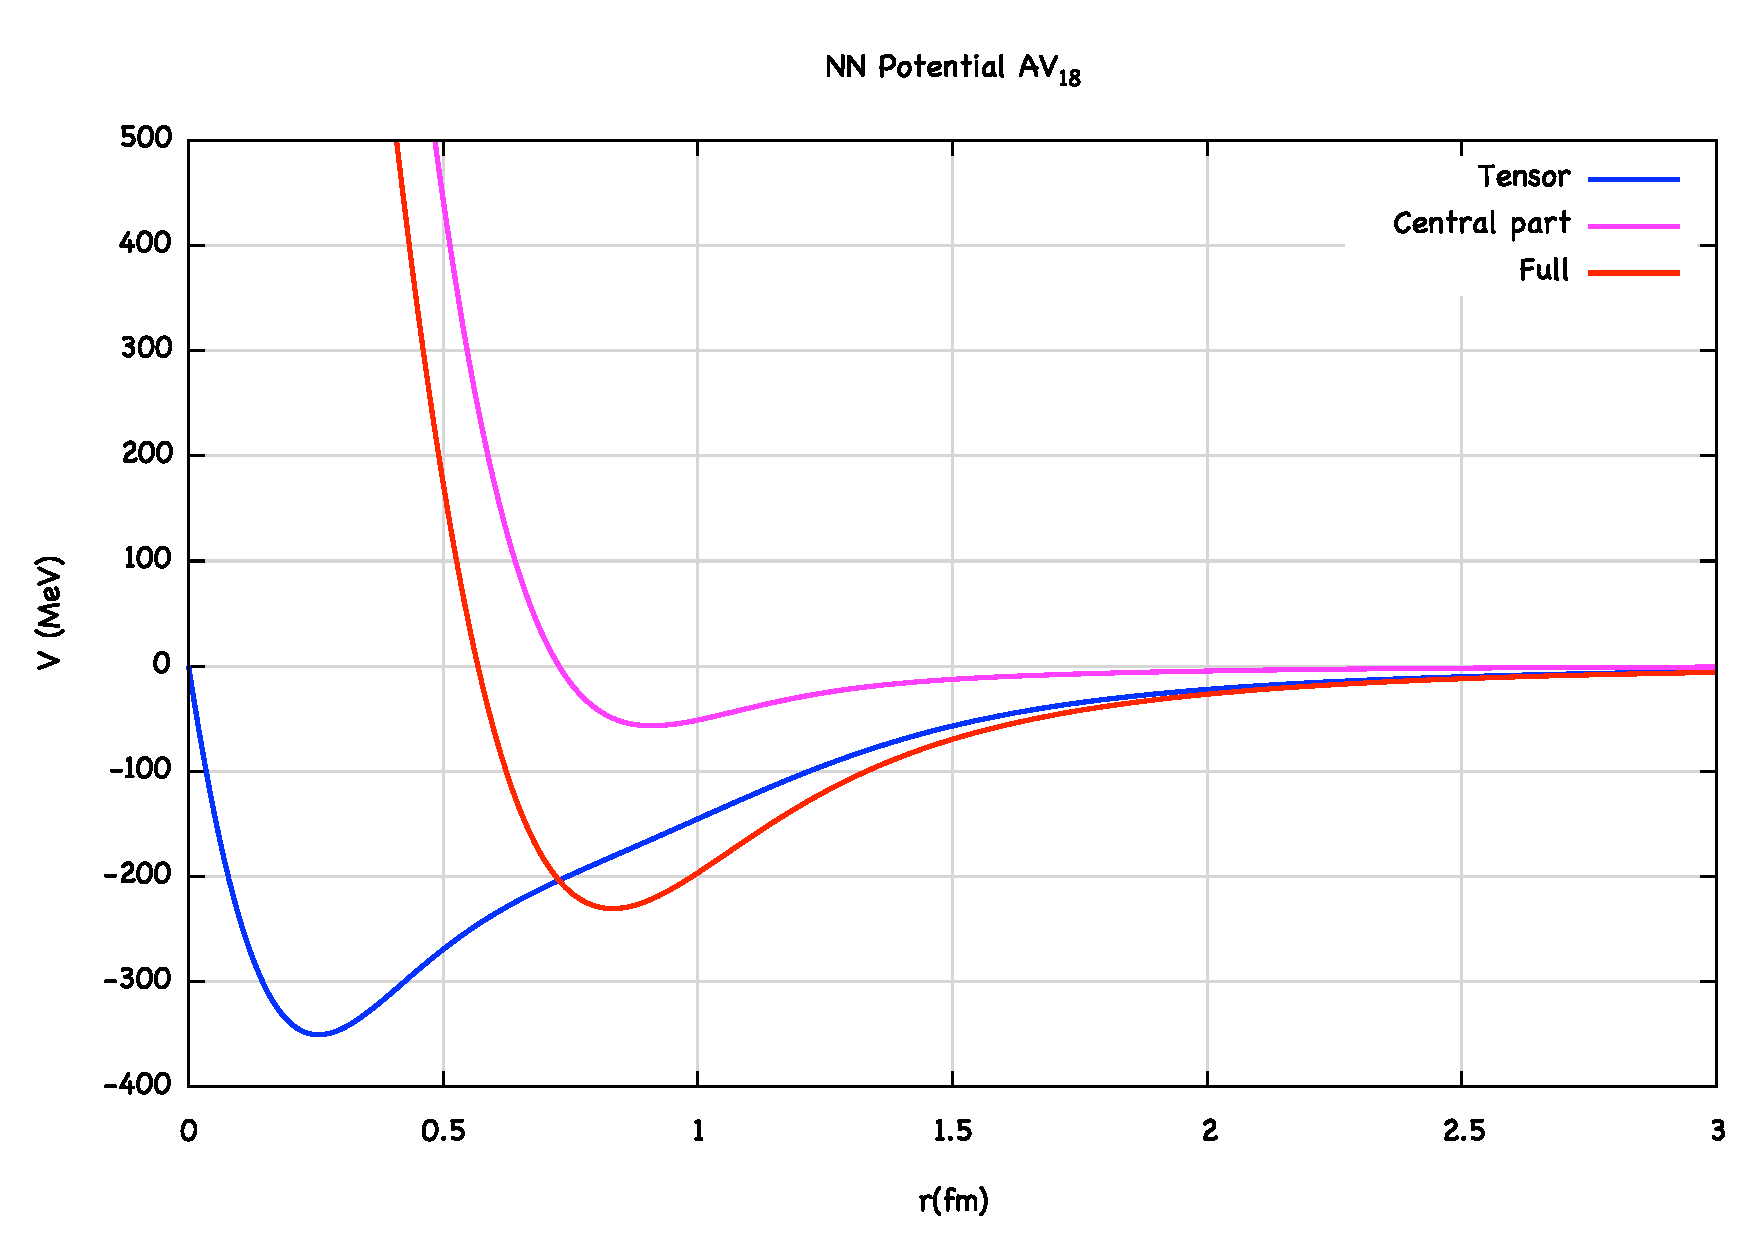
\includegraphics[type=pdf,ext=.pdf,read=.pdf,width=0.80\linewidth]{./figures/physics/CentralTensorFull}
    \caption[Two-nucleon interactions]{\footnotesize{Two-nucleon interactions calculated from the Argonne V14 potential~\cite{PhysRevC.51.38}, where the blue line represents the tensor force component, the cyan line is the central part and the red line is the total of these two combined. Figure is provided by Ref.~\cite{donal_prvt}.}}
    \label{potential_well}
  \end{center}
\end{figure}

Furthermore, the particular behaviour of the interaction potential between nucleons also increases the complexity of the nuclear system. A specific NN potential is shown in Fig.~\ref{potential_well}~\cite{PhysRevC.51.38}. The weak attractive interaction at moderate distance is generated by the exchange of virtual pions between nucleons. At short distance (e.g. $\mathrm{r\leq 1.5}$ fm), the interaction becomes strongly attractive on account of the tensor components of spin and isospin channels. At much shorter distance, the repulsive hard-core interaction between nucleons prevents the nucleus from collapsing. The Coulomb force between protons and potential three-body forces contribute but play a small role.

%\begin{figure}[!ht]
%  \begin{center}
%    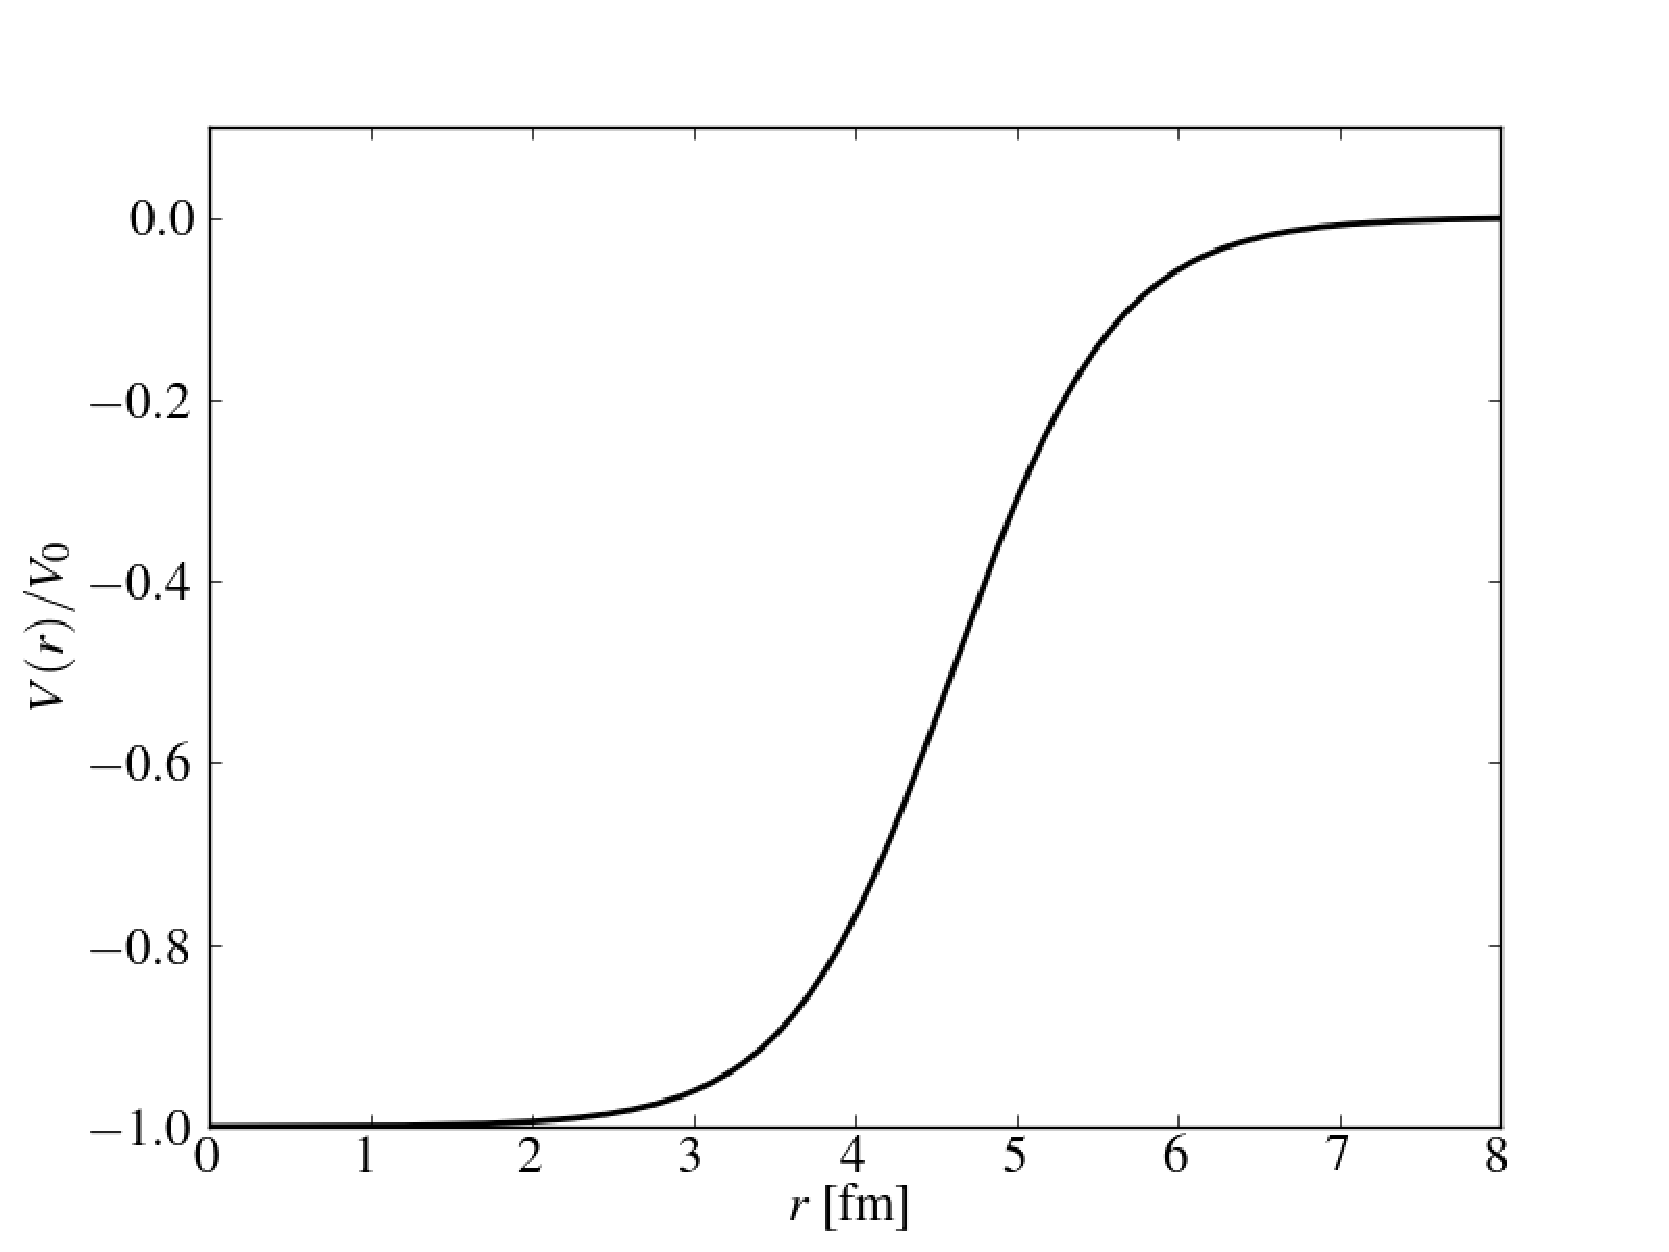
\includegraphics[type=pdf,ext=.pdf,read=.pdf,width=0.60\linewidth]{./figures/physics/Woods_Saxon_potential}
%    \caption[The Woods-Saxon potential]{\footnotesize{The Woods-Saxon potential~\cite{PhysRev.95.577}. Two nucleons only interact at long distance due to the exchange of pions. There is roughly no interaction at close distance. Figure is reproduced based on Ref.~~\cite{PhysRev.95.577}.}}
%    \label{woods_saxon}
%  \end{center}
%\end{figure}
Despite the complexity of the nucleus, studies have revealed that nucleons behave like independent particles in the nuclear medium due to the collective effects of the Pauli principle and the average interaction with surrounding nucleons. In this picture, nucleons weakly interact with each other at short distance, and nucleons tended to occupy discrete energy states similar to the arrangement of electrons orbiting around the nucleus. It was also found that some nuclei have much large binding energies when they are composed of certain numbers of nucleons, namely magic numbers. 

These phenomena have been successfully described by the independent particle shell model (IPSM), also called the mean field theory. In this theory, the nucleon is treated as a non-relativistic object and moves in an average field generated by surrounding nucleons, and the NN interactions between nucleons are ignored. Nucleons occupy the lowest energy states first. The momentum and energy of the last occupied state are called the Fermi momentum and Fermi energy, respectively, and the whole set of occupied energy levels is called the Fermi sea. The energy state of each nucleon can be individually obtained by solving the Schrodinger equation with the mean field potential. Combined with the spin-orbit coupling, the IPSM successfully predicts the ground state properties, the excitation of nuclei at low energy, nuclear spins and parities, as well as the magic numbers. 
  
 \begin{figure}[!ht]
  \begin{center}
    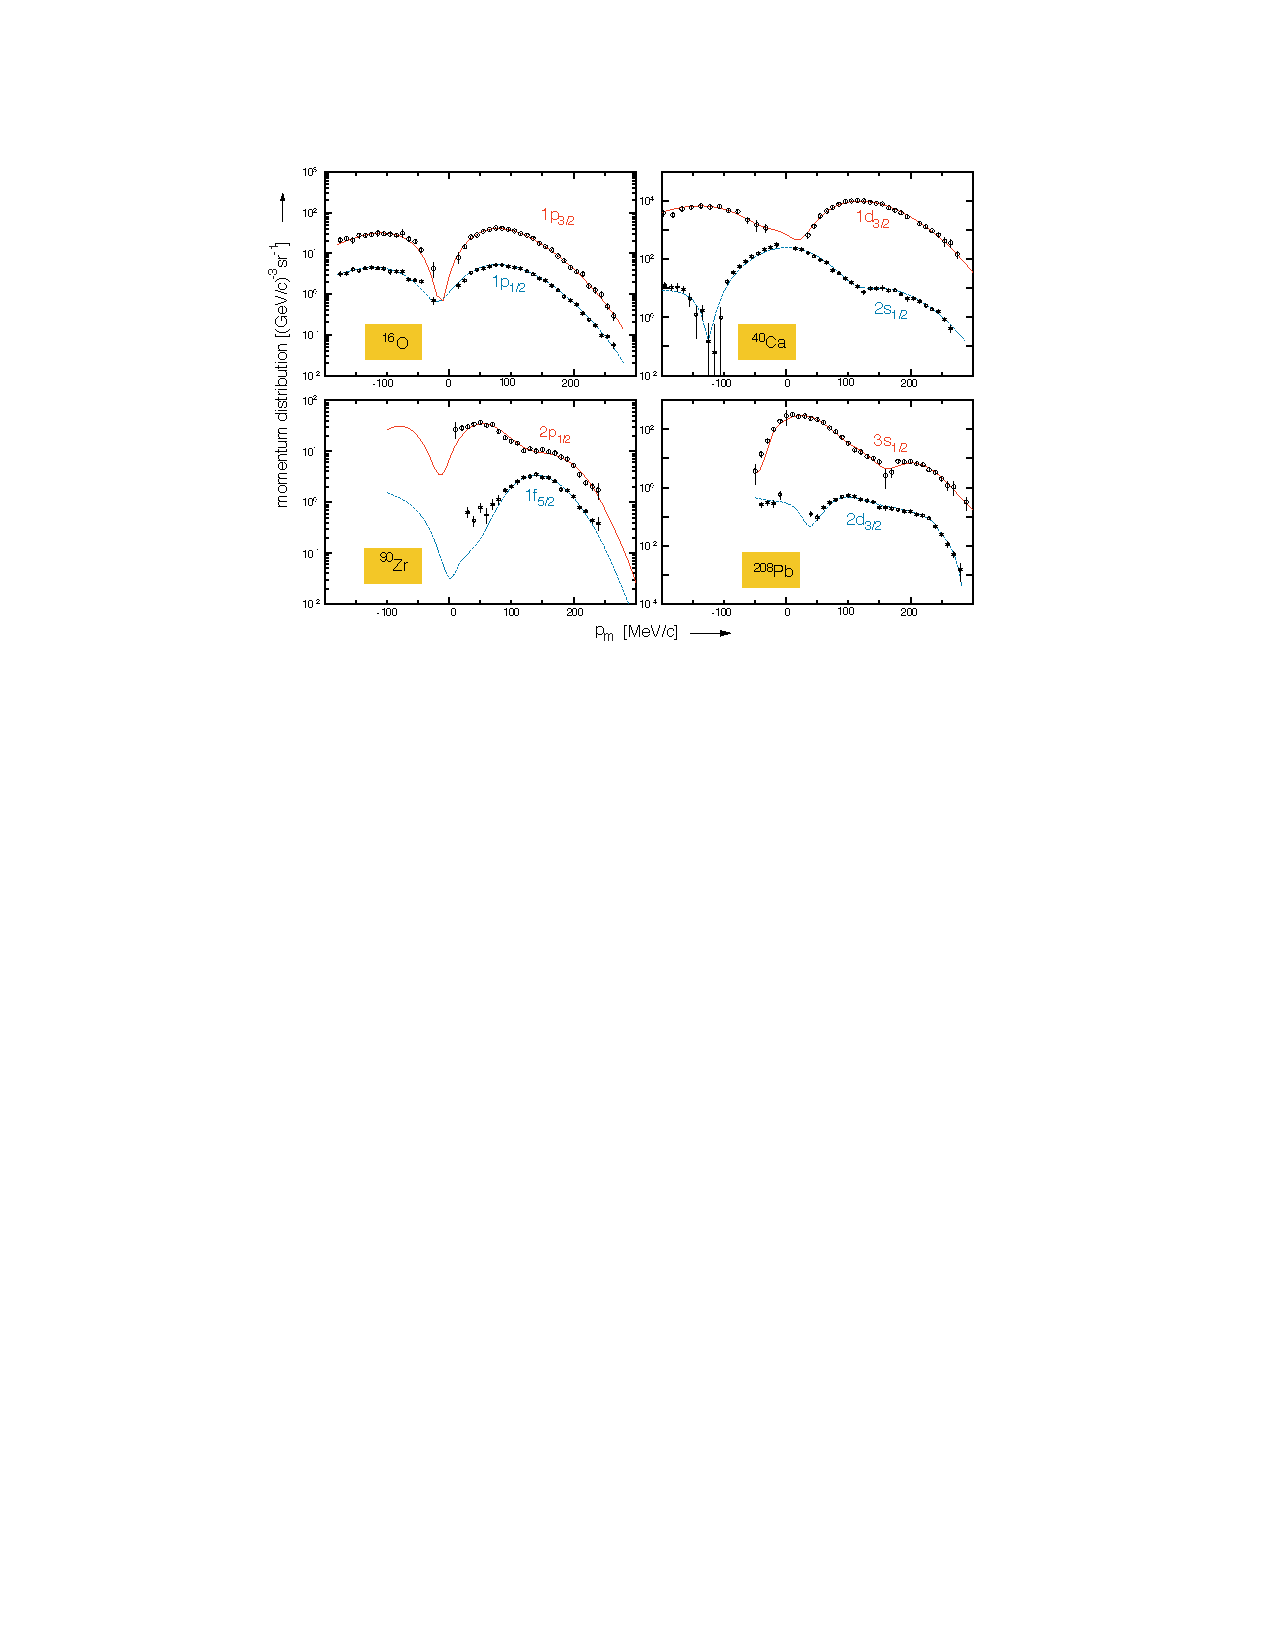
\includegraphics[type=pdf,ext=.pdf,read=.pdf,width=0.95\linewidth]{./figures/physics/Nikhefeep}
    \caption[Momentum distribution from NIKNEF data]{\footnotesize{Momentum distribution from NIKNEF data, where each plot denotes the momentum distribution of a nucleon in different shell inside a nucleus. Dots are the results of electron proton-knock-out measurements in NIKNEF and the lines are the theoretical calculation with DWIA. To agree with the data, a factor of 0.65 was applied to the DWIA calculation. Plot is from Ref.~\cite{VanDerSteenhoven1988547}}}
    \label{niknef_mom_dis}
  \end{center}
\end{figure} 
 Nevertheless, the IPSM shows its limitations in predicting the nuclear magnetic moments and highly excited energy states~\cite{review_mft}. Furthermore, discrepancies had been observed in high resolution medium-energy proton-knock-out reactions in the early 1970s. The electron scattering cross section measurements at NIKNEF~\cite{VanDerSteenhoven1988547} studied the momentum distribution for various shell model orbits. In the IPSM, the nucleon wave function was calculated through the impulse plane wave approximation (PWIA)~\cite{DeForest1983} with a simplified optical potential. Taking account of the medium effect, the distorted wave impulse approximation (DWIA)\footnote{The distorted wave impulse approximation (DWIA) is a non-relativistic model used at intermediate energies to compensate for the effects of a mean nuclear potential. Basic scattering reaction calculations often assume that the incident nucleon behaves as a plane wave till it interacts with the a nucleon in the nucleus. In fact, the potential field of the nucleus, which is usually given by an optical potential, will distort the nucleon wave function.} was used with a more complex potential, e.g. the Woods-Saxon potential. However, from the data shown in Fig.~\ref{niknef_mom_dis}, to agree with the experimental observations, the momentum distribution calculated from DWIA had to be scaled by a factor of 0.65, although the shape was well reproduced. Other advanced Hartree-Fock calculations attempted to resolve this discrepancy by involving the long range NN interactions but still overestimated the nuclear strength~\cite{hartree_fock_book}.

\begin{figure}[!ht]
  \begin{center}
    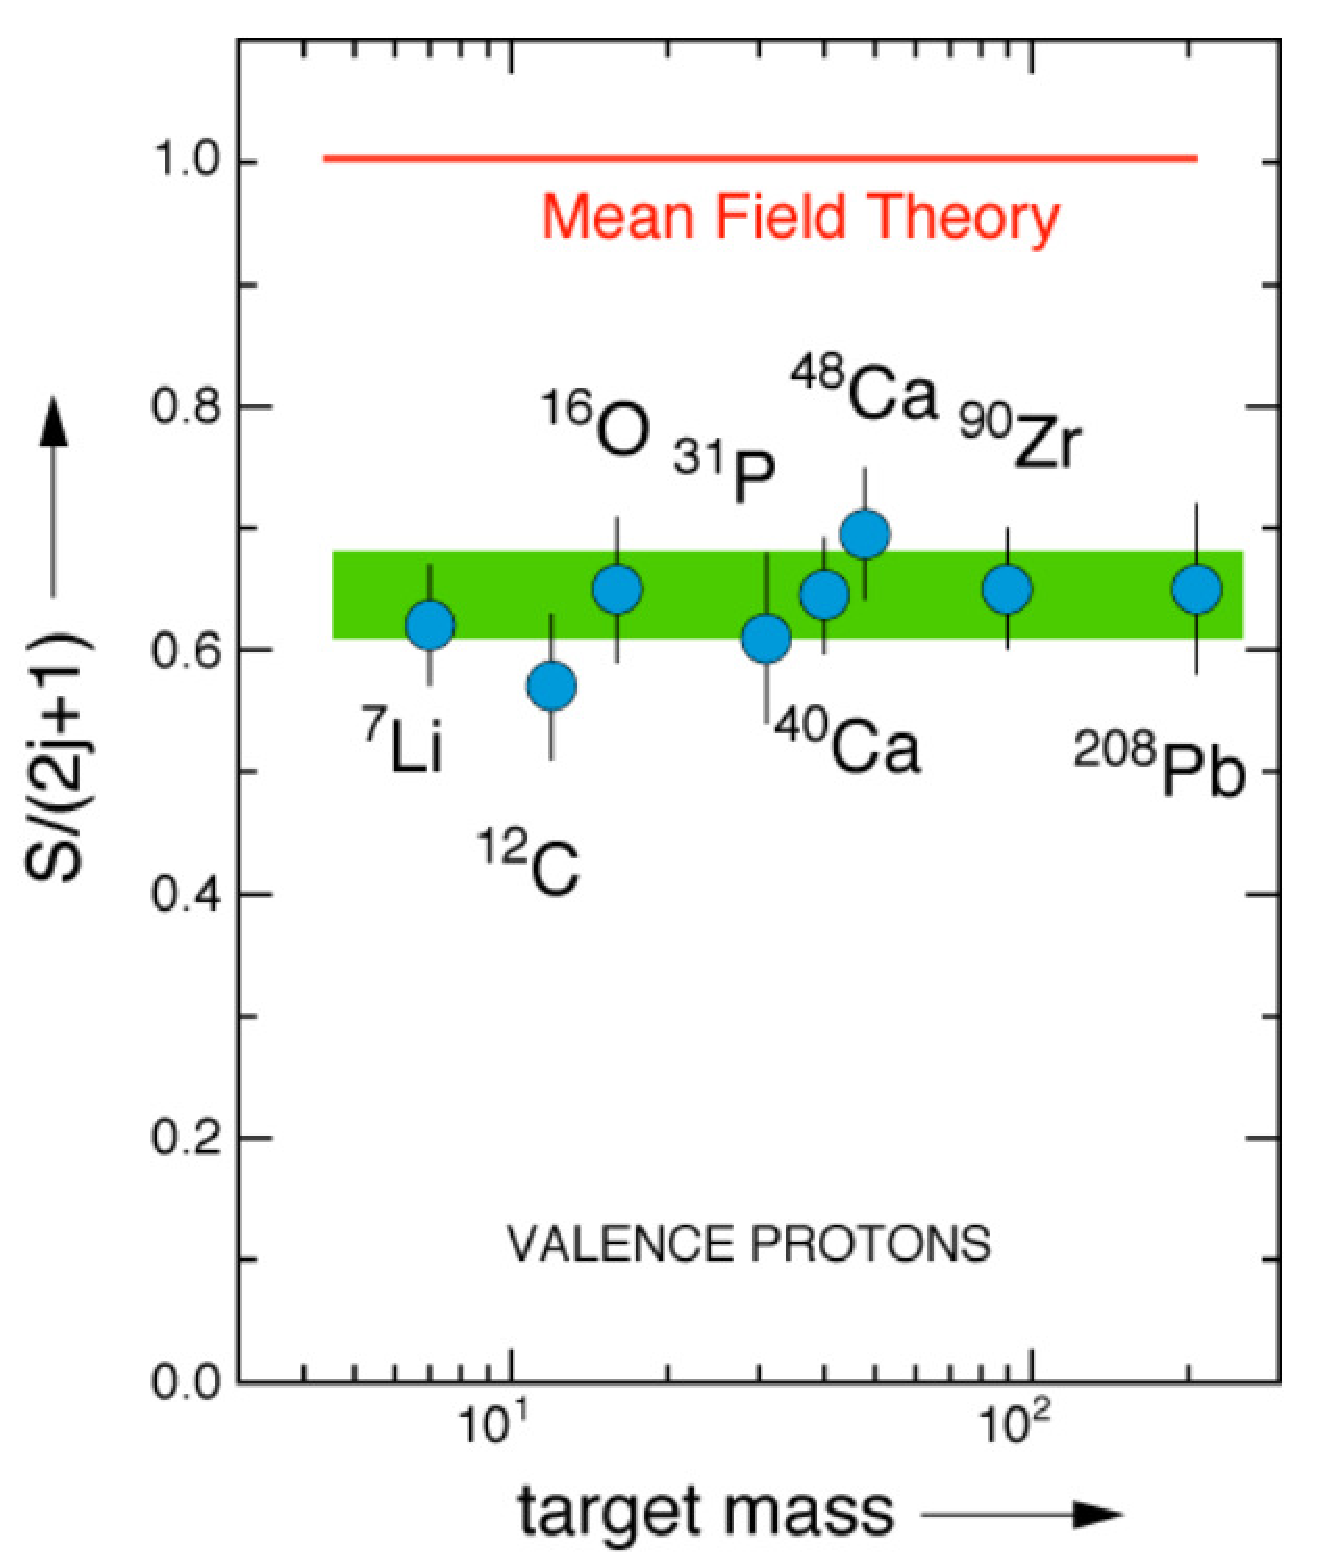
\includegraphics[type=pdf,ext=.pdf,read=.pdf,width=0.45\linewidth]{./figures/physics/spec_fac_exp}
    \caption[Measurements of spectroscopy factors]{\footnotesize{Measurements of spectroscopy factors for different nuclei deviate from one, where the y-axis denotes the ratio of the measured occupation number of a nucleon in a nucleus compared with the mean field prediction. The plot suggests that the mean field theory overestimates the occupation of a nucleon's states. Figure is from Ref.~\cite{Lapikas1993297}.}}
    \label{spec_fac_exp}
  \end{center}
\end{figure} 
 From these cross section measurements, one obtained the spectroscopic factors or the occupation numbers, and discovered that the occupancies of the same orbits were 30\%-40\% below the expected values~\cite{Lapikas1993297,Kelly:1996hd}, as shown in Fig.~\ref{spec_fac_exp}. 
 
 The missing nuclear strength can be understood by considering the short range NN interactions. The IPSM restricts nucleons in their energy states below the Fermi surface. However, as shown in Fig.~\ref{potential_well}, two nucleons do interact at short distance as a result of the attractive potential, and at much shorter distance, the repulsive force will push them apart. Taken together, it is realized that nucleons must carry high relative momenta which significantly exceed the Fermi momentum. Knock-out measurements revealed that the nuclear strength is beyond the predictions of the mean field. 
 
 Nucleons with high energies and momenta are generally referred to as short range correlations (SRC), which will be discussed in the next chapter.
